%%%%%%%%%%%%%%%%%%%%%%%%%%%%%%%%%%%%%%%%%%%%%%%%%%%%%%%%%%%%%%%
%\subsection{Task 2}
%\label{sub:task2}

Task 2 consists of extract all couples from a given model, either from Task 1 or IMBd database~\cite{imdbsources}. Two persons are couple whether they played together in at least three movies~\cite{imdbcase}. Once again we present the e-Motions and the Maude solution.

\subsubsection{e-Motions-based solution}

Fig.~\ref{fig:createCouple} shows the \code{createCouple} rule which implements the whole task. \code{Person} objects are shown using square shapes because \code{Person} is an abstract class and it does not have image attached. The \code{createCouple} rule consists of a LHS with a OCL condition, which states \textit{``LHS holds iff there are two persons \code{per1} and \code{per2}, such that the number of movies in the intersection between \code{per1}'s movies and \code{per2}'s movies is greater or equal than 3''}. Moreover, the \code{coupleHasNotBeenCreated} NAC avoids the application of the rule if the couple already exists. 

However, although this solution works, one can notice that the number of matchings in the LHS of the rule is combinatorial. The fact that there are such a large number of matchings makes this solution too inefficient. \todo{add numbers supporting this.}

\begin{figure}[htp]
  \centering
  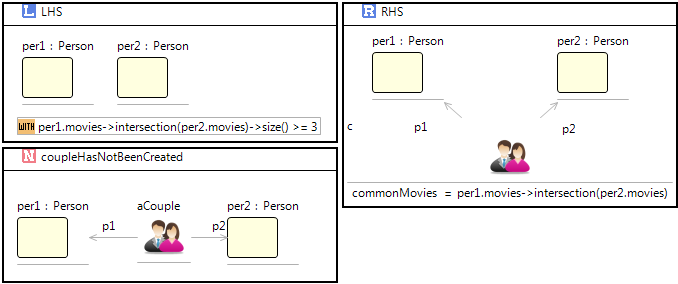
\includegraphics[width=\textwidth]{imgs/ruleCouples}
  \caption{\code{createCouple} rule.}\label{fig:createCouple}
\end{figure}

We have implemented another solution in which we limit the number of matchings using the next algorithm:
\begin{enumerate}
  \item We split \code{Person}s and \code{Movie}s into separate configurations.
  \item We fix a \code{Person}.
  \item Given a \code{Person}, we look for all couples.
  \item Whether the current \code{Person} set has been gone over all the other persons, we set the next person, and the current person is move to the resulting collection.
\end{enumerate}

Following this approach the number of persons to match as possible couple decrease. A new concept so-called \code{Collection} is added to the metamodel with its concrete syntax to implement the algorithm above mentioned. Fig.~\ref{fig:areCouples} shows one of the rules specified for this solution,\footnote{The rest of the rules are available at \url{https://github.com/antmordel/ttc14emotions}.} namely those that creates new couples. The box is the concrete syntax for the \code{Collection} concept.

\begin{figure}[htp]
  \centering
  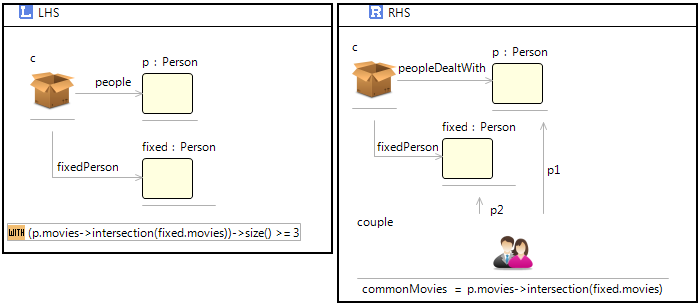
\includegraphics[width=\textwidth]{imgs/areCouple}
  \caption{\code{doingCouples} rule.}\label{fig:areCouples}
\end{figure}

\todo{add numbers}

\subsubsection{Maude-based solution}

